\clearpage

% Megjegyzések:
% \begin{outline}
%   \1 Ahol nincs kiírva mértékegység, ott az SI értendő.
%   \1 Az egységugrás függvényt $\theta(t)$-vel jelölöm.
% \end{outline}

A második házi feladat a tárgyhoz kapcsolódó első házi feladat folytatása.
A rendszer paraméterei és egyenleteit ott tárgyaltam, amelyeket itt fel fogok használni.

% {{{
\subsection*{Az egyenáramú motor paraméterei}

\begin{table}[H]
\begin{tabular}{llll}\toprule
Név                                & Jelölés           & Katalógus-beli érték                    & SI-beli érték                           \\ \midrule
armatúra ellenállás                & $\Ra$             & 11,1 $\Omega$                           & 11,1 $\Omega$                           \\
armatúra induktivitás              & $\La$             & 1,52 mH                                 & $1,52\cdot10^{-3}$ H                    \\
nyomatékállandó                    & $\km$             & 58,2 $\frac{\text{mNm}}{\text{V}}$      & 0,0582 $\frac{\text{Nm}}{\text{V}}$     \\
sebességállandó                    & $\ks$             & 164 $\frac{\text{rpm}}{\text{V}}$       & 17,17 $\frac{\text{rad}}{\text{Vs}}$    \\
elektromos állandó                 & $\ke$             & 0,006097  $\frac{\text{V}}{\text{rpm}}$ & 0,05822 $\frac{\text{Vs}}{\text{rad}}$  \\
forgórész tehetetlenségi nyomatéka & $\Ja$             & 44,6 $\text{gcm}^2$                     & 4,46$\cdot10^{-6}~\text{kgm}^2$         \\
névleges szögsebesség              & $\omega_\text{n}$ & 4430 rpm                                & 463,91 $\frac{\text{rad}}{\text{s}}$    \\
névleges áramerősség               & $i_\text{n}$      & 0,804 A                                 & 0,804 A                                 \\
névleges feszültség                & $u_\text{n}$      & 36 V                                    & 36 V                                    \\ \bottomrule
\end{tabular}
\caption{A motor és a hajtómű paraméterei}
\end{table}
%}}}

\begin{figure}[H]
	\centering
	\begin{subfigure}[H]{\textwidth}
		\centering
		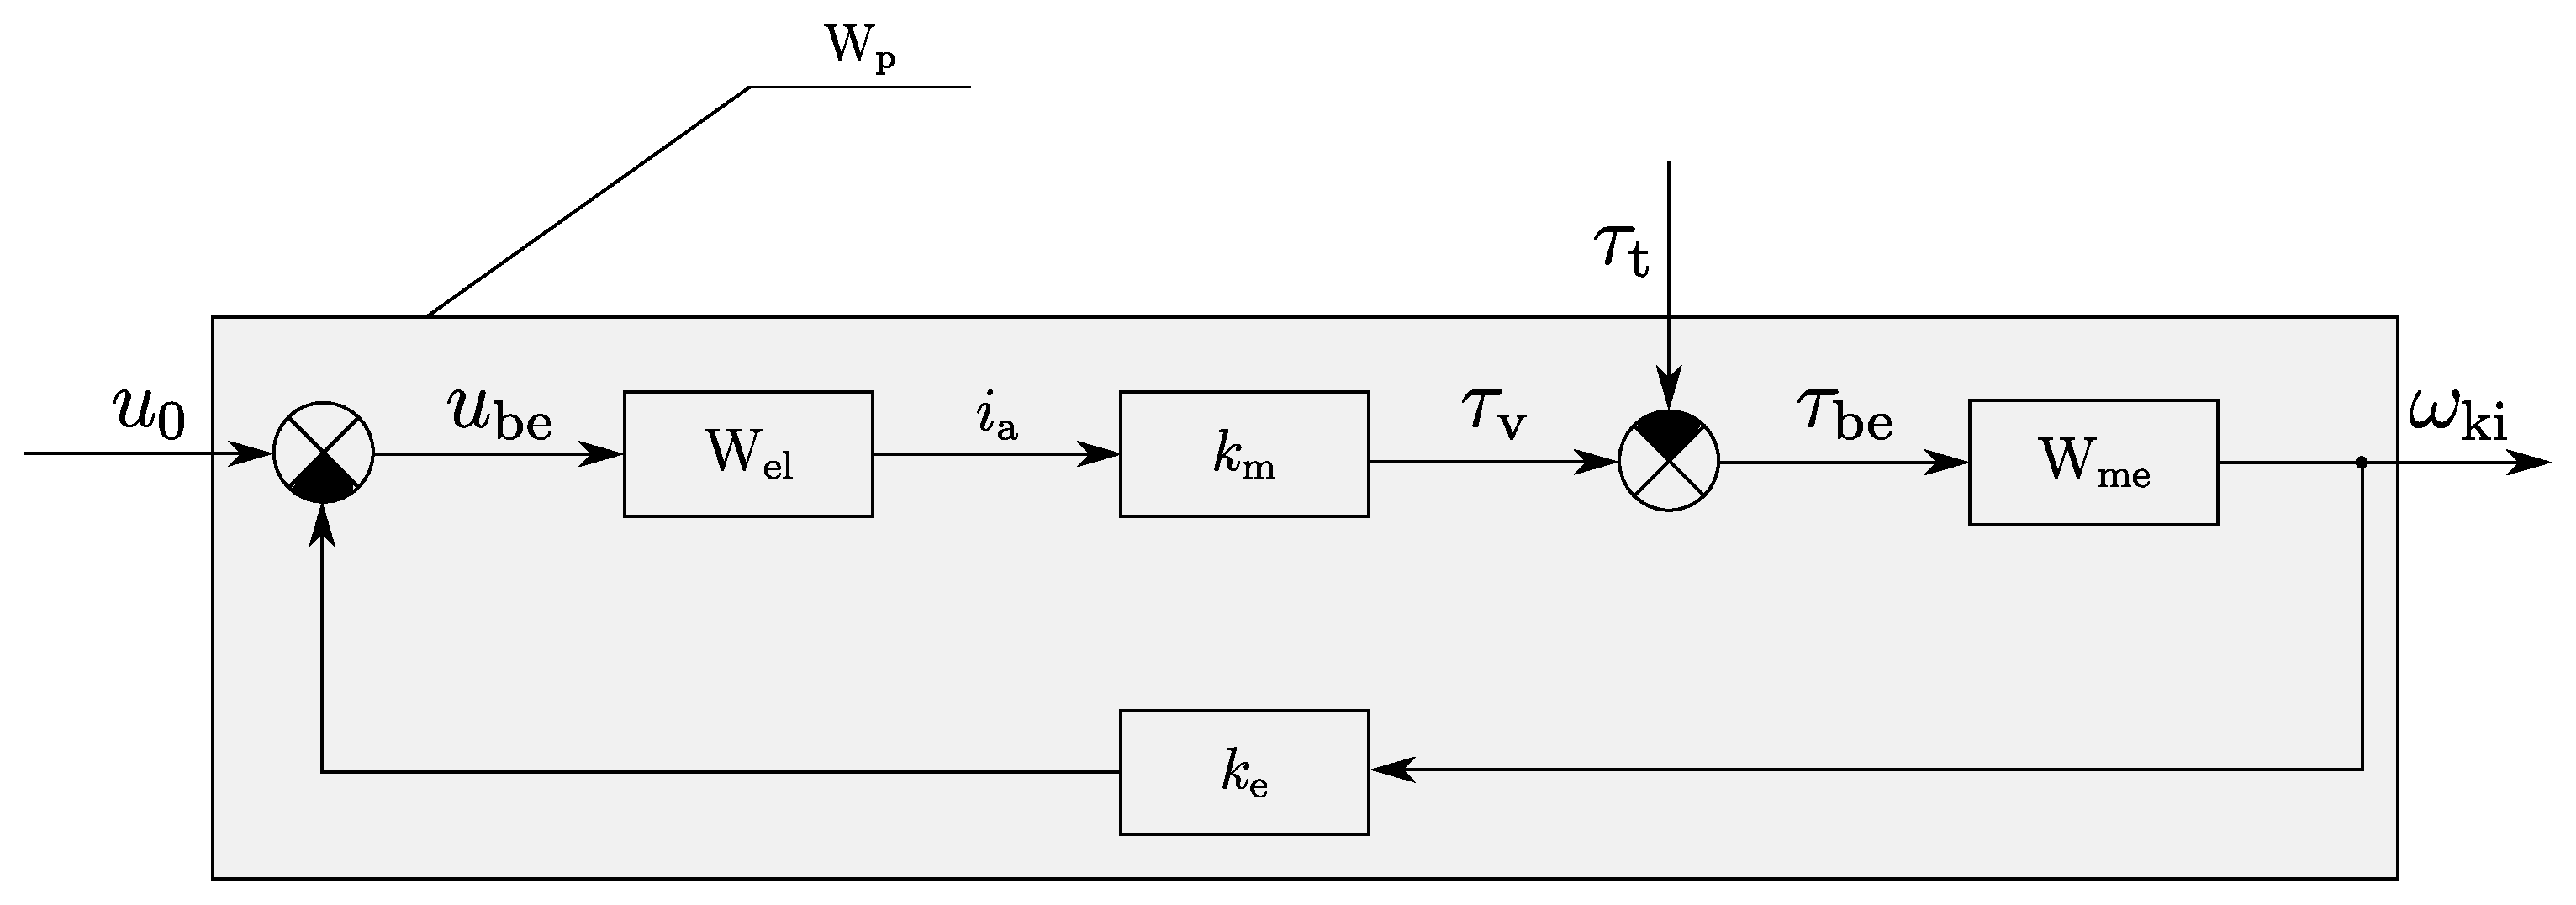
\includegraphics[width=.8\textwidth]{process-hatasvazlat}
		\caption{A motor hatásvázlata}
		\label{fig:process-hatasvazlat}
	\end{subfigure}\\[15mm]
	
	\begin{subfigure}[H]{\textwidth}
		\centering
		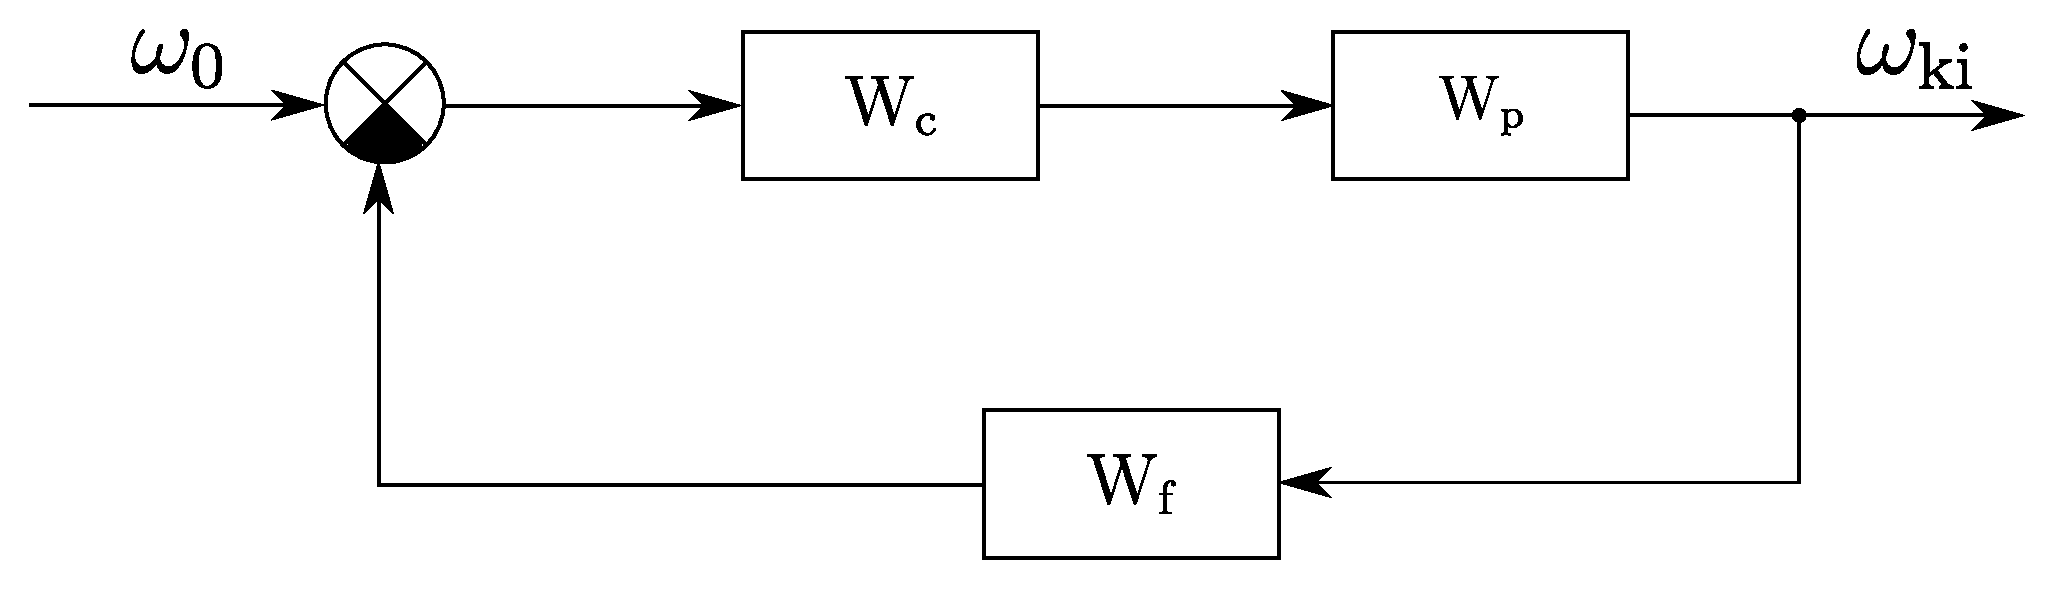
\includegraphics[width=.6\textwidth]{pi-hatasvazlat}
		\caption{A visszacsatolt rendszer hatásvázlata}
		\label{fig:pi-hatasvazlat}
	\end{subfigure}
	\caption{A szakasz és a teljes rendszer hatásvázlatai}
\end{figure}
